\section{Evaluation von Segmentierungsergebnissen}

\begin{defi}{Metrik}
    % TODO: https://de.wikipedia.org/wiki/Metrischer_Raum#Einordnung_in_die_Hierarchie_mathematischer_Strukturen 
    Sei $X$ eine beliebige Menge.
    Eine Abbildung $d: X \times X \to \mathbb {R}$ heißt \emph{Metrik} auf $X$, wenn für beliebige Elemente $x, y, z \in \mathbb{R}$ die folgenden Eigenschaften gelten:
    \begin{itemize}
        \item Positive Definitheit: $d(x, y) \geq 0$ und $d(x, y) = 0 \iff x = y$.
        \item Symmetrie: $d(x, y) = d(y, x)$
        \item Dreiecksungleichung: $d(x, y) \leq d(x, z) + d(z, y)$
    \end{itemize}
\end{defi}

\begin{defi}{Wahrheitsmatrix}
    % TODO: https://de.wikipedia.org/wiki/Beurteilung_eines_bin%C3%A4ren_Klassifikators#Wahrheitsmatrix:_Richtige_und_falsche_Klassifikationen 
    Um einen Klassifikator zu bewerten, muss man ihn in einer Reihe von Fällen anwenden, bei denen man zumindest im Nachhinein Kenntnis über die \enquote{wahre} Klasse der jeweiligen Objekte hat.
    Dabei können vier mögliche Fälle auftreten:
    \begin{itemize}
        \item \emph{Richtig positiv} (engl. true positive, \emph{TP})
        \item \emph{Falsch negativ} (engl. false negative, \emph{FN})
        \item \emph{Falsch positiv} (engl. false positive, \emph{FP})
        \item \emph{Richtig negativ} (engl. true negative, \emph{TN})
    \end{itemize}

    Es wird nun gezählt, wie häufig jede der vier möglichen Kombinationen von ermittelter Klasse und tatsächlicher Klasse vorgekommen ist.
    Diese Häufigkeiten werden in eine sogenannte \emph{Wahrheitsmatrix} (auch Konfusionsmatrix genannt) eingetragen:

    TODO: Tabelle

    \centering
    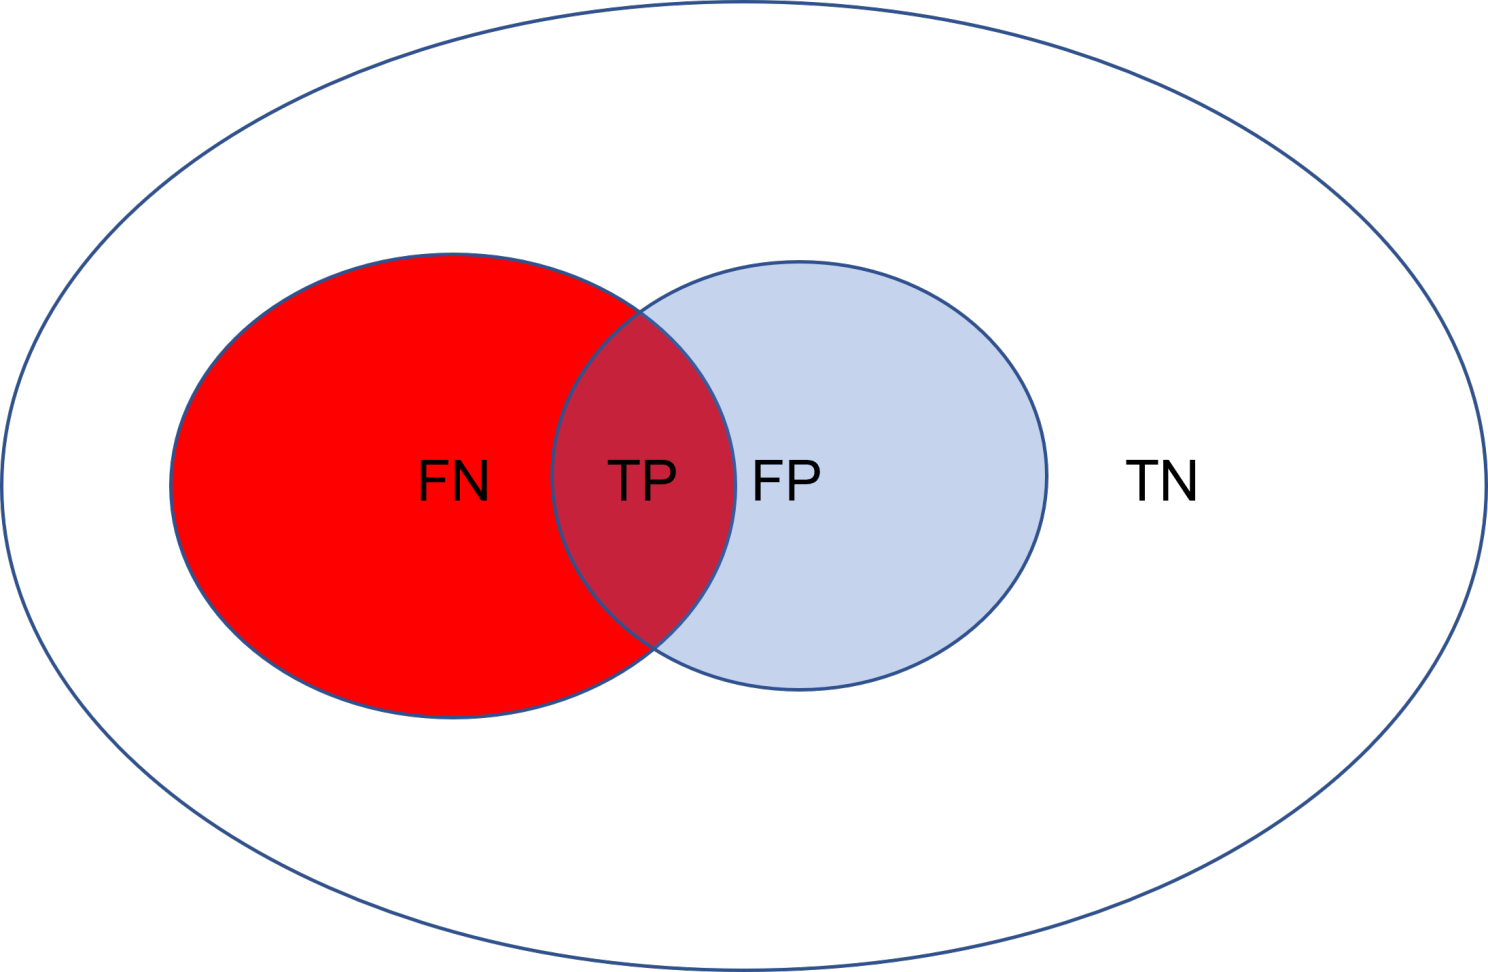
\includegraphics[width=.5\linewidth]{figures/wahrheitsmatrix_venn.png}
\end{defi}

\begin{defi}[Überlappungsmetrik]{Jaccard-Koeffizient}
    % TODO: https://de.wikipedia.org/wiki/Jaccard-Koeffizient 
    Der \emph{Jaccard-Koeffizient} oder \emph{Jaccard-Index}, auch \emph{Intersection over Union} ist eine Kennzahl für die Ähnlichkeit von Mengen.

    Um den Jaccard-Koeffizient zweier Mengen zu berechnen, teilt man die Anzahl der gemeinsamen Elemente (Schnittmenge) durch die Größe der Vereinigungsmenge:
    \[
        J(A, B) = \frac{|A \cap B|}{|A \cup B|}
    \]
    Je näher der Jaccard-Koeffizient an $1$ liegt, desto größer ist die Ähnlichkeit der Mengen.
    Der minimale Wert des Jaccard-Koeffizienten ist $0$.
\end{defi}

\begin{bonus}[Überlappungsmetrik]{DICE-Koeffizient}
    Der \emph{DICE-Koeffizient} berechnet sich als zweimal die Schnittmenge geteilt durch die Summe der Kardinalitäten der einzelnen Mengen.
    \[
        D(A, B) = \frac{2 \cdot |A \cap B|}{|A| +  |B|}
    \]

    DICE lässt sich in Jaccard ausdrücken und umgekehrt.
    Beide Metriken messen die gleichen Aspekte.
\end{bonus}

\begin{defi}[Überlappungsmetrik]{Sensitivität}
    Die \emph{Sensitivität} (auch \emph{Richtig-positiv-Rate}; engl. \emph{Sensitivity}, \emph{True Positive Rate}, \emph{Recall} oder \emph{Hit Rate}) gibt die Wahrscheinlichkeit an, mit der ein positives Objekt korrekt als positiv klassifiziert wird.

    Beispielsweise bedeutet eine Sensitivität eines Tests auf ein Virus von 98 \%, dass (bei ausreichend großer Anzahl an durchgeführten Tests und unabhängig von den Testvorbedingungen) 98 \% der Infizierten erkannt und 2 \% der Infizierten nicht erkannt würden.
    2 \% (der Infizierten, welche getestet wurden, und nicht aller Getesteten) wären dann also falsch negativ.

    Die Sensitivität entspricht der geschätzten bedingten Wahrscheinlichkeit:
    \[
        \text{Sensitivity} = P(\text{positives Testergenis} \mid \text{tatsächlich krank}) = \text{TPR} = \frac{\text{TP}}{\text{TP} + \text{FN}}
    \]

    Die Sensitivität ist empfindlich bzgl. der Größe der Ergebnismengen.
    Fehler in kleinen Ergebnismengen werden stärker betont, als in großen Ergebnismengen.

    TODO: Venn-Diagramm
\end{defi}

\begin{defi}[Überlappungsmetrik]{Spezifizität}
    Die \emph{Spezifität} (auch \emph{Richtig-negativ-Rate}; engl. \emph{Specificity}, \emph{True Negative Rate}) gibt die Wahrscheinlichkeit an, mit der ein negatives Objekt korrekt als negativ klassifiziert wird.

    % Beispielsweise entspricht die Spezifität bei einer medizinischen Diagnose dem Anteil an Gesunden, bei denen auch festgestellt wurde, dass keine Krankheit vorliegt. 
    % Die Spezifität eines Tests gibt an, mit welcher Wahrscheinlichkeit ein Nicht-Infizierter auch tatsächlich erkannt würde. 

    Beispielsweise bedeutet eine Spezifität eines Tests auf ein Virus von 98 \%, dass (bei ausreichend großer Anzahl an durchgeführten Tests und unabhängig von den Testvorbedingungen) 98 \% der Nicht-Infizierten tatsächlich erkannt und 2 \% der Nicht-Infizierten fälschlich als infiziert ausgewiesen würden.
    2 \% (der getesteten Nicht-Infizierten, nicht der Getesteten insgesamt) wären dann also falsch positiv.

    Die Spezifität entspricht der geschätzten bedingten Wahrscheinlichkeit:
    \[
        \text{Specificity} = P(\text{negatives Testergenis} \mid \text{tatsächlich gesund}) = \text{TNR} = \frac{\text{TN}}{\text{TN} + \text{FP}}
    \]

    Die Spezifizität ist empfindlich bzgl. der Größe der Ergebnismengen.
    Fehler in kleinen Ergebnismengen werden stärker betont, als in großen Ergebnismengen.

    TODO: Venn-Diagramm
\end{defi}

\begin{bonus}[Überlappungsmetrik]{False-positiv-Rate}
    Die \emph{Falsch-positiv-Rate} lässt sich aus der Spezifizität ableiten:
    \[
        FPR = 1 - \text{Specificity} = \frac{\text{FP}}{\text{FP} + \text{TN}}
    \]

    TODO: Venn-Diagramm
\end{bonus}

\begin{bonus}[Überlappungsmetrik]{False-negativ-Rate}
    Die \emph{Falsch-negativ-Rate} lässt sich aus der Sensitivität ableiten:
    \[
        FNR = 1 - \text{Sensitivity} = \frac{\text{FN}}{\text{FN} + \text{TP}}
    \]

    TODO: Venn-Diagramm
\end{bonus}

\begin{defi}[Überlappungsmetrik]{Positive Predictive Value}
    Der \emph{positive Vorhersagewert} (engl. \emph{Positive Predictive Value}, \emph{PPV}) gibt den Anteil der korrekt als positiv klassifizierten Ergebnisse an der Gesamtheit der als positiv klassifizierten Ergebnisse an:
    \[
        \text{Specificity} = \text{PPV} = \frac{\text{TP}}{\text{TP} + \text{FP}}
    \]
\end{defi}

\begin{defi}[Überlappungsmetrik]{Negative Predictive Value}
    Der \emph{negative Vorhersagewert} (engl. \emph{Negative Predictive Value}, \emph{NPV}) gibt den Anteil der korrekt als negativ klassifizierten Ergebnisse an der Gesamtheit der als negativ klassifizierten Ergebnisse an:
    \[
        \text{NPV} = \frac{\text{TN}}{\text{TN} + \text{FN}}
    \]
\end{defi}

\begin{defi}[Entfernungsmetrik]{Hausdorff-Distanz}
    % TODO: https://de.wikipedia.org/wiki/Hausdorff-Metrik
    Die \emph{(symmetrische) Hausdorff-Distanz} misst den Abstand $\delta(A, B)$ zwischen nichtleeren kompakten Teilmengen $A$, $B$ eines metrischen Raums $E$.

    Anschaulich haben zwei kompakte Teilmengen einen geringen Hausdorff-Abstand, wenn es zu jedem Element der einen Menge ein Element der anderen Menge gibt, zu dem dieses einen geringen Abstand hat.

    Als Hilfsmittel definiert man den Abstand $D$ zwischen einem Punkt $x$ und einer nichtleeren kompakten Teilmenge $K \subseteq E$ unter Rückgriff auf die Metrik $d$ des Raums $E$ als
    \[
        D(x, K) := \min \{ d(x, k) \mid k \in K \}
    \]

    Dann definiert man den Hausdorff-Abstand zwischen zwei nichtleeren kompakten Teilmengen $A$ und $B$ als
    \[
        \delta(A, B) := \max \{ \max \{ D(a, B) \mid a \in A \}, \{ D(b, A) \mid b \in B \} \}
    \]

    Die symmetrische Hausdorff-Distanz lässt sich nicht effizient mit Brute Force bestimmen.
    Besser funktionieren Nearest-Neighbor-Algorithmen.
\end{defi}

\begin{defi}[Entfernungsmetrik!Hausdorff-Distanz]{Gerichtete Hausdorff-Distanz}
    Die \emph{gerichtete Hausdorff-Distanz} ist die größte Distanz einer Menge $A$ zum nächsten Element einer anderen Menge $B$ bzgl. einer Norm $d$.
    \[
        h(A, B) := \max_{a \in A} \{ \min_{b \in B} \{ d(A, B) \}  \}
    \]

    Die gerichtete Hausdorff-Distanz ist asymmetrisch.

    Die gerichtete Hausdorff-Distanz lässt sich effizient per Brute Force bestimmen.
\end{defi}

\begin{defi}[Entfernungsmetrik!Hausdorff-Distanz]{Durchschnittliche Hausdorff-Distanz}
    Die \emph{durchschnittliche Hausdorff-Distanz} ist weniger empfindlich gegenüber Ausreißern und definiert als
    \[
        h(A, B) := \frac{1}{N} \sum_{a \in A} \min_{b \in B} \{ d(A, B) \}
    \]
\end{defi}